\documentclass[a4paper]{article}
\usepackage[a4paper,margin=0mm]{geometry}
\usepackage{fontspec}
\usepackage{unicode-math}
\usepackage{tikz}
\usetikzlibrary{fit,calc,positioning}
\usepackage[table]{xcolor}
\usepackage[absolute]{textpos}
\usepackage{array}

\setmainfont{Libertinus Serif}
\setsansfont{Libertinus Sans}
\setmathfont{Libertinus Math}

\definecolor{accent}{HTML}{F46530}
\definecolor{badge}{HTML}{FFBDA5}
\definecolor{ink}{HTML}{2A2E30}

\setlength{\TPHorizModule}{1mm}
\setlength{\TPVertModule}{1mm}
\setlength{\parindent}{0pt}
\pagestyle{empty}

\newcommand{\topicheader}[2]{%
\begin{textblock*}{194mm}(16mm,10mm)
\begin{tikzpicture}
\node[fill=accent,text=white,font=\sffamily\bfseries\fontsize{13}{13}\selectfont,
      minimum width=9mm,minimum height=9mm,inner sep=0pt] at (4.5mm,-4.5mm) {#1};
\node[font=\sffamily\bfseries\fontsize{15}{16}\selectfont,text=ink,anchor=west] at (12mm,-4.5mm) {#2};
\end{tikzpicture}
\end{textblock*}
\begin{textblock*}{194mm}(16mm,22.5mm)

\begin{tikzpicture}
\fill[accent] (0,0) rectangle (194mm,0.5mm);
\end{tikzpicture}
\end{textblock*}
}

\newcommand{\pagekicker}[1]{%
\begin{textblock*}{100mm}(16mm,25.5mm)
\begin{tikzpicture}
\node[fill=ink,text=white,font=\sffamily\bfseries\fontsize{8}{8}\selectfont,
      inner sep=2.2pt,rounded corners=1pt] {\MakeUppercase{#1}};
\end{tikzpicture}
\end{textblock*}
}

\newcommand{\pagefooter}[1]{%
\begin{textblock*}{194mm}(8mm,286.41mm)
  
\begin{tikzpicture}
    \fill[accent] (0,0) rectangle (194mm,0.6mm);
  \end{tikzpicture}
\end{textblock*}
\begin{textblock*}{63.59mm}(8mm,288.27mm)
  {\sffamily\bfseries\color{accent}\fontsize{13}{16}\selectfont SAT 1200+}
\end{textblock*}
\begin{textblock*}{10mm}(188mm,288.27mm)
  \centering{\sffamily\color{accent}\fontsize{14}{16}\selectfont #1}
\end{textblock*}
}

\newcommand{\cardbg}[4]{%
\begin{textblock*}{#3mm}(#1mm,#2mm)
\begin{tikzpicture}
\fill[badge!22,rounded corners=3mm] (0,0) rectangle (#3mm,-#4mm);
\end{tikzpicture}
\end{textblock*}%
}

\newcommand{\pill}[3]{%
\begin{textblock*}{160mm}(#1mm,#2mm)
\begin{tikzpicture}
\node[fill=accent,text=white,anchor=north west,font=\sffamily\bfseries\fontsize{10}{10}\selectfont,
      rounded corners=8pt,inner xsep=5mm,inner ysep=1.8mm] at (0,0) {QOIDA ~\textperiodcentered~ #3};
\end{tikzpicture}
\end{textblock*}%
}

\arrayrulecolor{accent}
\setlength{\arrayrulewidth}{0.7pt}
\renewcommand{\arraystretch}{1.5}

\begin{document}

\topicheader{5}{Algebraik ifodalar}
\pagekicker{Formula sheet}
\pagefooter{37}
\mbox{}%

% ================= CARD 1: Had, koeffitsient, o'xshash hadlar (y: 33-103) =================
\cardbg{16}{33}{178}{70}
\pill{26}{36}{Had, koeffitsient, o'xshash hadlar}

\begin{textblock*}{158mm}(26mm,52mm)
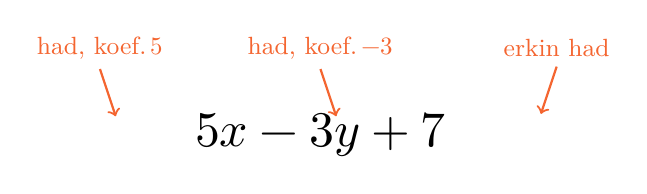
\begin{tikzpicture}
\node[font=\fontsize{18}{18}\selectfont] (expr) at (0,0) {$5x-3y+7$};
\node[font=\fontsize{9}{10}\selectfont,text=accent] (l1) at (-28mm,11mm) {had, koef.\,$5$};
\node[font=\fontsize{9}{10}\selectfont,text=accent] (l2) at (0mm,11mm) {had, koef.\,$-3$};
\node[font=\fontsize{9}{10}\selectfont,text=accent] (l3) at (30mm,11mm) {erkin had};
\draw[accent,->,line width=0.8pt] (l1.south) -- ++(2mm,-6mm);
\draw[accent,->,line width=0.8pt] (l2.south) -- ++(2mm,-6mm);
\draw[accent,->,line width=0.8pt] (l3.south) -- ++(-2mm,-6mm);
\end{tikzpicture}
\end{textblock*}

\begin{textblock*}{158mm}(26mm,80mm)
\begin{tikzpicture}[every node/.style={font=\fontsize{13}{13}\selectfont}]
\node[anchor=west] at (0,0) {$4x+3y-x+7$};
\node[anchor=west,font=\fontsize{12}{12}\selectfont] at (52mm,0) {$\xrightarrow{\ x\text{ hadlarni qo'shing}\ }$};
\node[anchor=west,font=\sffamily\bfseries\fontsize{13}{13}\selectfont,text=accent] at (105mm,0) {$3x+3y+7$};
\end{tikzpicture}
\end{textblock*}

% ================= CARD 2: Taqsimot xossasi (y: 109-184) =================
\cardbg{16}{109}{178}{75}
\pill{26}{112}{Taqsimot xossasi}

\begin{textblock*}{158mm}(26mm,128mm)
\begin{center}
{\fontsize{17}{17}\selectfont $a(b+c)=ab+ac$}
\end{center}
\end{textblock*}

\begin{textblock*}{158mm}(26mm,142mm)
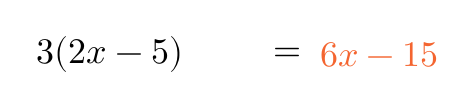
\begin{tikzpicture}[every node/.style={font=\fontsize{13}{13}\selectfont}]
\node[anchor=west] at (0,0) {$3(2x-5)$};
\node[anchor=west] at (30mm,0) {$=$};
\node[anchor=west,font=\sffamily\bfseries\fontsize{13}{13}\selectfont,text=accent] at (36mm,0) {$6x-15$};
\end{tikzpicture}
\end{textblock*}

\begin{textblock*}{158mm}(26mm,158mm)
{\fontsize{9.5}{12}\selectfont\color{black!60}Manfiy ishora qavsdagi \textbf{har bir} hadga tatbiq etiladi:}
\end{textblock*}

\begin{textblock*}{158mm}(26mm,167mm)
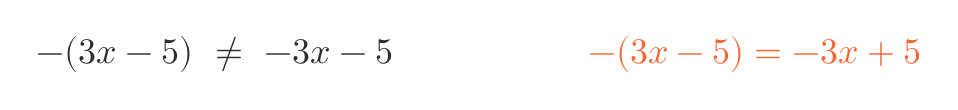
\begin{tikzpicture}[every node/.style={font=\fontsize{13}{13}\selectfont}]
\node[anchor=west,text=ink] at (0,0) {$-(3x-5)\ \ne\ -3x-5$};
\node[anchor=west,font=\sffamily\bfseries\fontsize{13}{13}\selectfont,text=accent] at (70mm,0) {$-(3x-5)=-3x+5$};
\end{tikzpicture}
\end{textblock*}

% ================= CARD 3: Ko'p hadli ifodani soddalashtirish (y: 190-275) =================
\cardbg{16}{190}{178}{85}
\pill{26}{193}{Ko'p hadli ifodani soddalashtirish}

\begin{textblock*}{158mm}(26mm,210mm)
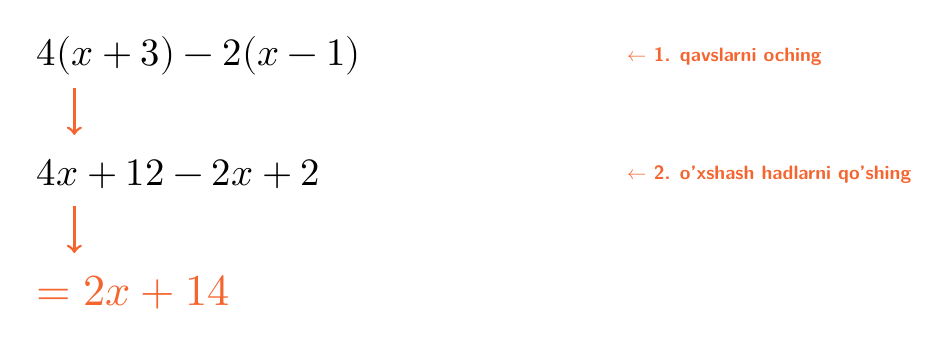
\begin{tikzpicture}[every node/.style={font=\fontsize{14}{14}\selectfont}]
\node[anchor=west] (l0) at (0,0) {$4(x+3)-2(x-1)$};
\node[anchor=west,font=\sffamily\bfseries\scriptsize,text=accent] at (75mm,0) {$\leftarrow$ 1. qavslarni oching};

\node[anchor=west] (l1) at (0,-15mm) {$4x+12-2x+2$};
\node[anchor=west,font=\sffamily\bfseries\scriptsize,text=accent] at (75mm,-15mm) {$\leftarrow$ 2. o'xshash hadlarni qo'shing};

\node[anchor=west,font=\sffamily\bfseries\fontsize{16}{16}\selectfont,text=accent] (l2) at (0,-30mm) {$=2x+14$};

\foreach \y in {-4,-19}{
  \draw[accent,->,line width=1pt] (6mm,\y mm) -- (6mm,\y mm -6mm);
}
\end{tikzpicture}
\end{textblock*}

\begin{textblock*}{158mm}(26mm,252mm)
{\fontsize{9}{11}\selectfont\color{black!55}\itshape Har bir qavs taqsimot xossasi bilan alohida ochiladi (manfiy ishoraga e'tibor bering), keyin o'xshash hadlar ixchamlanadi.}
\end{textblock*}

\end{document}
